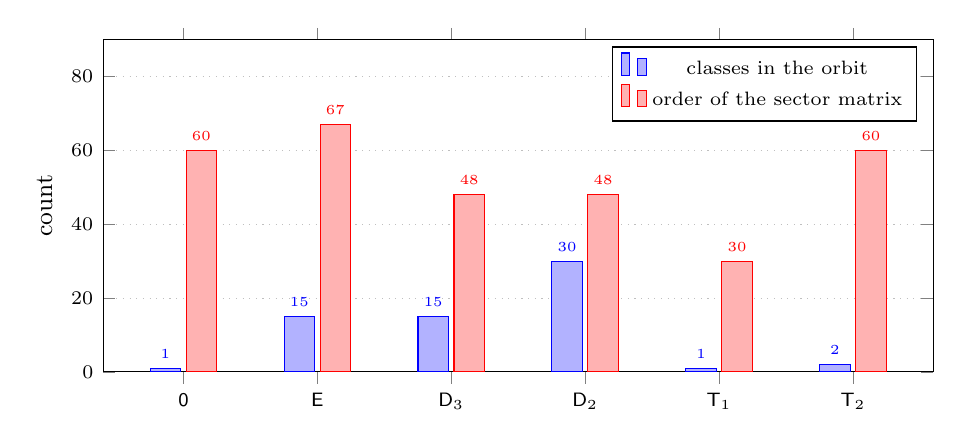
\begin{tikzpicture}
\begin{axis}[ybar,width=\textwidth,height=5.8cm,bar width=11pt,ymin=0,ymax=90,symbolic x coords={0,E,D3,D2,T1,T2},xtick=data,xticklabels={$\mathsf{0}$,$\mathsf{E}$,$\mathsf{D}_3$,$\mathsf{D}_2$,$\mathsf{T}_1$,$\mathsf{T}_2$},ylabel={count},tick label style={font=\scriptsize},label style={font=\small},legend style={font=\scriptsize,at={(0.98,0.98)},anchor=north east},enlarge x limits=0.12,nodes near coords,nodes near coords style={font=\tiny},point meta=y,ymajorgrids=true,grid style={dotted}]
\addplot coordinates {(0,1) (E,15) (D3,15) (D2,30) (T1,1) (T2,2)};
\addplot coordinates {(0,60) (E,67) (D3,48) (D2,48) (T1,30) (T2,60)};
\legend{classes in the orbit,order of the sector matrix}
\end{axis}
\end{tikzpicture}
